\begin{figure}[t]
\subfigure[Impact of varying passage number to retrieval]{
\begin{minipage}[t][2.5cm][t]{0.46\linewidth}
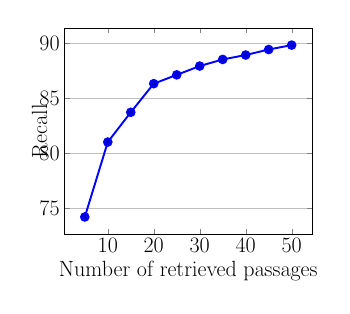
\begin{tikzpicture}[scale=0.46]
    \begin{axis}[
        xlabel=Number of retrieved passages,
        ylabel=Recall,
        y label style={at={(-0.05,0.5)}},
        ymajorgrids=true,
        % xlabel style={text width=8cm},
        font=\LARGE,
        ]
        \addplot+[color=blue,line width=1.5pt,mark size=3pt] coordinates {
            (5,74.2)
            (10,81.0)
            (15,83.7)
            (20,86.3)
            (25,87.1)
            (30,87.9)
            (35,88.5)
            (40,88.9)
            (45,89.4)
            (50,89.8)
        };
    \end{axis}
\end{tikzpicture}
\label{fig:q3-3-1}
\end{minipage}
}
\subfigure[Impact of varying passage number to HC-LLM]{
\begin{minipage}[t][2.5cm][t]{0.46\linewidth}
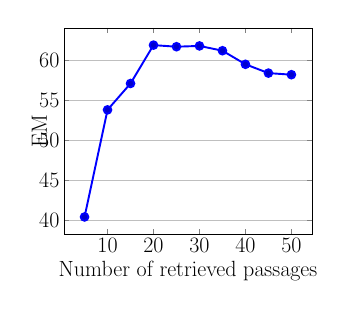
\begin{tikzpicture}[scale=0.46]
    \begin{axis}[
        xlabel=Number of retrieved passages,
        ylabel=EM,
        y label style={at={(-0.05,0.5)}},
        ymajorgrids=true,
        font=\LARGE,
        % ymin=0.12,
        % ymax=0.18,
        ]
        \addplot+[color=blue,line width=1.5pt,mark size=3pt] coordinates {
            (5,40.4)
            (10,53.8)
            (15,57.1)
            (20,61.9)
            (25,61.7)
            (30,61.8)
            (35,61.2)
            (40,59.5)
            (45,58.4)
            (50,58.2)
        };
    \end{axis}
\end{tikzpicture}
\label{fig:q3-3-2}
\end{minipage}
}
\caption{Impact of retrieved passage number}
\end{figure} 
